\documentclass{article}
\usepackage[top=1cm,left=1cm,right=1.5cm,bottom=2cm]{geometry}
\usepackage[utf8]{inputenc}
\title{Algorithm Homework}
\author{Tai Jiang}
\date{October 2023}
\usepackage{hyperref}
\usepackage{tcolorbox}
\usepackage{amsmath}
\usepackage{amssymb}
\usepackage{tikz}
\usepackage{color}
\usepackage{listings}
\lstset{
 columns=fixed,       
 numbers=left,                                        % 在左侧显示行号
 language=c++,                                        % 设置语言
}

\begin{document}
  \maketitle
  \tableofcontents
  \pagenumbering{gobble}
  \newpage
  \pagenumbering{arabic}
  \section{Show that the solution of  $ T \left(n\right) = T \left(\left\lceil n/2 \right\rceil\right) + 1  $ is $ O \left( \lg n \right)  $ .}
    \paragraph{Origin}:
      \subparagraph{Exercise}4.3-2
      \subparagraph{Page}87
    \paragraph{Answer}:

  That can build a recursion tree to visualize how this recurrence works:

  \begin{enumerate}
    \item Start with $ T \left(n\right) $ at the top.
    \item At each level of the tree, we have $ T \left( \left\lceil n/2 \right\rceil \right) + 1 $.
    \item The tree branches into two subproblems, one with size $ \left\lceil n/2 \right\rceil $ and another with size $ \left\lceil n/2 \right\rceil $.
  \end{enumerate}

  The tree might look like Figure \ref{fig:tree1}.

  \begin{figure}[h!]
    \centering
    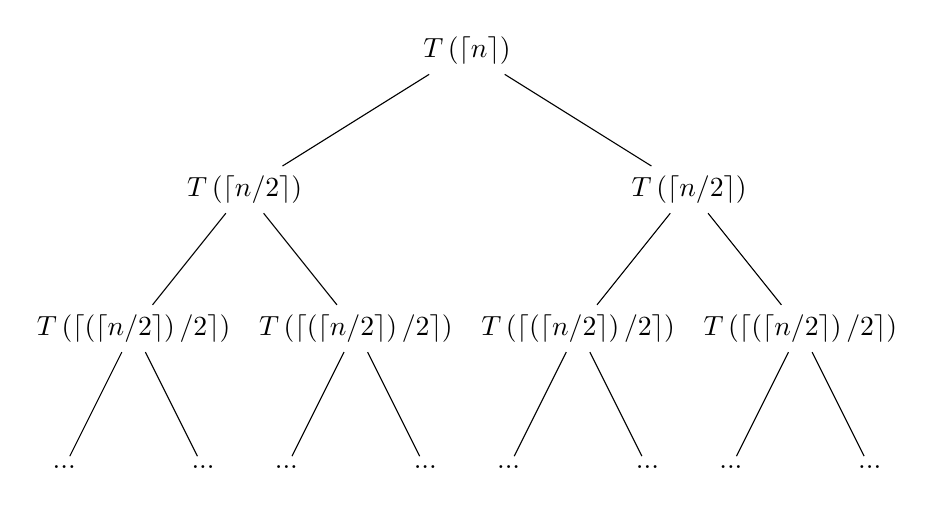
\begin{tikzpicture}
      [level distance=50px,
       level 1/.style={sibling distance=160px},
       level 2/.style={sibling distance=80px},
       level 3/.style={sibling distance=50px}]
      \node {$ T \left(\left\lceil n \right\rceil\right) $}
        child {node {$ T \left(\left\lceil n/2 \right\rceil\right) $}
          child {node {$ T \left(\left\lceil  \left(\left\lceil n/2 \right\rceil\right) /2 \right\rceil\right) $}
            child {node {...}}
            child {node {...}}
          }
          child {node {$ T \left(\left\lceil  \left(\left\lceil n/2 \right\rceil\right) /2 \right\rceil\right) $}
            child {node {...}}
            child {node {...}}
          }
        }
        child {node {$ T \left(\left\lceil n/2 \right\rceil\right) $}
          child {node {$ T \left(\left\lceil  \left(\left\lceil n/2 \right\rceil\right) /2 \right\rceil\right) $}
            child {node {...}}
            child {node {...}}
          }
          child {node {$ T \left(\left\lceil  \left(\left\lceil n/2 \right\rceil\right) /2 \right\rceil\right) $}
            child {node {...}}
            child {node {...}}
          }
        };
    \end{tikzpicture}
    \caption{Recursion Tree.}
    \label{fig:tree1}
  \end{figure}

  At each level, the size of the problem is divided by 2, and we keep going until the size becomes 1 (or less, in which case we stop). The depth of the tree will be the number of times we can halve n until it becomes 1. So it's the number of times we can take $ \left\lceil n/2 \right\rceil $ until $ \left\lceil n/2 \right\rceil \leq  1 $.
  
  At each step, we're taking the ceiling of half of the previous value, which is effectively dividing it by 2. We continue this process until the value is less than or equal to 1. So, let k be the number of steps it takes for $ \left\lceil n/2 \right\rceil $ to become 1, look like equation \eqref{eq:tree1}.

  \begin{equation}
    \frac{\left\lceil n/2 \right\rceil}{2^k}  \leq 1
    \label{eq:tree1}
  \end{equation}

  Then sovle for k, look like equation \eqref{eq:tree2}:
  
  \begin{equation}
    \begin{aligned}
      \frac{n}{2^k} \leq 1 \\
      n \leq 2^k \\
      \lg n \leq k
    \end{aligned}
    \label{eq:tree2}
  \end{equation}

  The depth of the recursion tree is $ O(\lg n) $, which means the algorithm has a time complexity of $ O(\lg n) $. So the solution of  $ T \left(n\right) = T \left(\left\lceil n/2 \right\rceil\right) + 1 $ is indeed $ O(\lg n) $.

  \section{Use a recursion tree to determine a good asymptotic upper bound on the recurrence $ T \left(n\right) = 4T \left( n/2 + 2 \right) + n  $. Use the substitution method to verify your answer.}
    \paragraph{Origin}:
      \subparagraph{Exercise}4.4-3
      \subparagraph{Page}93
    \paragraph{Answer}:

    That can build a recursion tree to visualize how this recurrence works:

    \begin{enumerate}
      \item Start with $ T \left(n\right)  $ at the top.
      \item At each level of the tree, we have 4 subproblems of size $ T \left( n/2 + 2 \right) + n  $.
      \item The cost of each level is n.
    \end{enumerate}

    The tree might look like Figure \ref{fig:tree2}.

  \begin{figure}[h!]
    \centering
    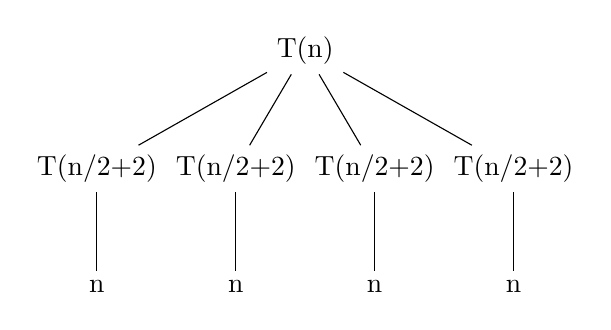
\begin{tikzpicture}[sibling distance=50px]
      \node {T(n)}
        child {node {T(n/2+2)}
          child {node {n}}
        }
        child {node {T(n/2+2)}
          child {node {n}}
        }
        child {node {T(n/2+2)}
          child {node {n}}
        }
        child {node {T(n/2+2)}
          child {node {n}}
        };

    \end{tikzpicture}
    \caption{Recursion Tree.}
    \label{fig:tree2}
  \end{figure}

  At each level, we have 4 subproblems of size T(n/2 + 2), and each subproblem incurs a cost of n. The number of levels in the tree will depend on how quickly the subproblem size decreases.

  The subproblem size is equation \eqref{eq:q2_1}:

  \begin{equation}
    T(n) = 4T(n/2 + 2) + n
    \label{eq:q2_1}
  \end{equation}

  The subproblem size is n/2 + 2, so we calculate the subproblem size for the next level by equation \eqref{eq:q2_2}:
  \begin{equation}
    \begin{aligned}
      T(n/2 + 2) &= 4T((n/2 + 2)/2 + 2) + n/2 + 2 \\
      &= 4T(n/4 + 1 + 2) + n/2 + 2 \\
      &= 4T(n/4 + 3) + n/2 + 2      
    \end{aligned}
    \label{eq:q2_2}
  \end{equation}

  At each level, we are adding 2 to the subproblem size. Therefore, at level k, the subproblem size will be $ n/(2^k) + 2k $.

  Now, we want to find the level where the subproblem size becomes a constant, $ n/(2^k) + 2k = C for some constant C $, calculate the k look like equation \eqref{eq:q2_3}.

  \begin{equation}
    \begin{aligned}
      n/(2^k) + 2k &= C \\
      n/(2^k) &= C - 2k \\
      2^k &= n/(C - 2k) \\
      k &= \lg (n/(C - 2k))
    \end{aligned}
    \label{eq:q2_3}
  \end{equation}

  C is a constant. The number of levels in the recursion tree is $ O(\lg n) $.

  The cost at each level in the recursion tree is equation \eqref{eq:q2_4}:

  \begin{equation}
    \begin{aligned}
      \text{At level 0:}& \quad n \\
      \text{At level 1:}& \quad 4 * n/2 = 2n \\
      \text{At level 2:}& \quad 4 * (n/4) = n \\
      ... \\
      \text{At level k:}& \quad (4^k) * (n/(2^k)) = (n/2^k) * (4^k) = C * 4^k
    \end{aligned}
    \label{eq:q2_4}
  \end{equation}

  Summing up the costs of all levels(Equation \eqref{eq:q2_5}):

  \begin{equation}
    T(n) = n + 2n + 4n + ... + C * 4^k
    \label{eq:q2_5}
  \end{equation}

  This is a geometric series, and its sum can be bounded by(Equation \eqref{eq:q2_6}):

  \begin{equation}
    T(n) \leq  n * (1 - 4^(k+1))/(1 - 4)
    \label{eq:q2_6}
  \end{equation}

  Since $k = O(\lg(n))$, $4^(k+1)$ is polynomial in n. Therefore, T(n) is O(n).

  verify this result using the substitution method:

  Assume that $T(m) \leq  km - p$ for some positive constants k and p, where m < n(Equation \eqref{eq:q2_7}).

  \begin{equation}
    \begin{aligned}
      T(n) = 4T(n/2 + 2) + n \\
        \leq  4(k(n/2 + 2) - p) + n \\
        = 2kn - 4k + 4n - 4p + n \\
        = (2k + 5)n - 4k - 4p
    \end{aligned}
    \label{eq:q2_7}
  \end{equation}

  Find k and p such that $(2k + 5)n - 4k - 4p \leq  kn - p$.
  
  This holds if $2k + 5 \leq k and -4k - 4p \leq -p$.
  
  Solving these inequalities(Equation \eqref{eq:q2_8}):

  \begin{equation}
    \begin{aligned}
      2k + 5 &\leq k \\
      k &\leq -5 \\
      -4k - 4p &\leq -p \\
      -4k &\leq 0\\
      k &\geq  0
    \end{aligned}
    \label{eq:q2_8}
  \end{equation}

  Since we can't find k and p that satisfy these inequalities, our initial assumption that $ T(m) \leq km - p$ for m < n is incorrect.

  Therefore, T(n) is not $O(n^k)$ for any positive constant k. Instead, as shown earlier, T(n) is O(n).
  
  \section{Can the master method be applied to the recurrence $ T(n) = 4T(n/2) + n^2 \lg n $? Why or why not? Give an asymptotic upper bound for this recurrence.}

  \paragraph{Origin}:
    \subparagraph{Exercise}4.5-4
    \subparagraph{Page}97
  \paragraph{Answer}:

  The master theorem can be applied to recurrence

  To apply the master theorem, we need to check whether f(n) satisfies the following conditions for some constant $\epsilon  > 0$:

  \begin{enumerate}
    \item If $ f(n) = O(n^{log_{b} a - \epsilon } ) $, for some $\epsilon > 0$, then $T(n) = \Theta (n^{log_{b}a})$.
    \item If $ f(n) = \Theta(n^{log_{b}a}) $, then $ T(n) = \Theta(n^{log_{b} a}  \lg n) $.
    \item If $ f(n) = \Omega (n^{log_{b}a + \epsilon}) $, for some $\epsilon > 0$, and if $a f(n/b) \leq k * f(n)$ for some k < 1 and sufficiently large n, then $T(n) = \Theta(f(n))$.
  \end{enumerate}

  The asymptotic upper bound for the given recurrence relation $T(n) = 4T(n/2) + n^2 * \lg n = O(n^2)$.

  \section{Use indicator random variables to compute the expected value of the sum of n dice.}

  \paragraph{Origin}:
    \subparagraph{Exercise}5.2-3
    \subparagraph{Page}122
  \paragraph{Answer}:

Let $X_i$ be the random variable that is 1 if the i-th die shows a particular face (1, 2, 3, 4, 5, or 6), and 0 otherwise.

The sum of n dice can then be expressed as the sum of these indicator variables:

$ S = X_1 + X_2 + X_3 + ... + X_n $

Now, we can calculate the expected value of S:

$ E(S) = E(X_1) + E(X_2) + E(X_3) + ... + E(X_n) $

Since each die is fair, the probability of each face (1, 2, 3, 4, 5, or 6) appearing on a single die is 1/6, and the expected value of each indicator variable is:

$ E(X_i) = 1 * P(X_i = 1) + 0 * P(X_i = 0) = 1 * (1/6) + 0 * (5/6) = 1/6 $

Now, you can sum up the expected values of the individual indicators:

$ E(S) = E(X_1) + E(X_2) + E(X_3) + ... + E(X_n) = (1/6) + (1/6) + (1/6) + ... + (1/6) = (n/6) $

So, the expected value of the sum of n dice is (n/6).



  \section{Use indicator random variables to solve the following problem, which is known as the hat-check problem. Each of n customers gives a hat to a hat-check person at a restaurant. The hat-check person gives the hats back to the customers in a random order. What is the expected number of customers who get back their own hat?}

  \paragraph{Origin}:
    \subparagraph{Exercise}5.2-4
    \subparagraph{Page}122
  \paragraph{Answer}:

  Let $X_i$ be an indicator random variable for the i-th customer, where:

  $X_i = 1$ if the i-th customer gets their own hat back.
  $X_i = 0$ if the i-th customer does not get their own hat back.
  
  The probability that the i-th customer gets their own hat back is 1/n, as there are n hats and they are returned in a random order. Therefore, we have:
  
  $E(X_i) = P(X_i = 1) = 1/n$
  
  Now, let's define a random variable Y as the total number of customers who get their own hat back. Y is the sum of the indicator random variables for each customer:
  
  $Y = X_1 + X_2 + X_3 + ... + X_n$
  
  Now, we can find the expected value of Y using linearity of expectation:
  
  $E(Y) = E(X_1 + X_2 + X_3 + ... + X_n)$
  
  Using the linearity of expectation, we can write this as:
  
  $E(Y) = E(X_1) + E(X_2) + E(X_3) + ... + E(X_n)$
  
  Since each customer's indicator random variable has the same expected value (1/n), we can simplify further:
  
  $E(Y) = (1/n) + (1/n) + (1/n) + ... + (1/n) (n times)$
  
  $E(Y) = (1/n) * n = 1$
  
  So, the expected number of customers who get back their own hat is 1. This result may be surprising, but it's a classic result of the hat-check problem. On average, one customer is expected to get their own hat back, while the others get hats belonging to other customers.
  \section{Show that the worst-case running time of HEAPSORT is $ \Omega (n \lg n)$.}
  \paragraph{Origin}:
    \subparagraph{Exercise}6.6-4
    \subparagraph{Page}160
  \paragraph{Answer}:

  Basic heapsort:

  \begin{enumerate}
    \item Build a max-heap from the input array.
    \item Repeatedly remove the maximum element from the heap and place it at the end of the array, shrinking the heap size.
    \item Repeat step 2 until the heap is empty.
  \end{enumerate}

  The worst-case occurs when the input array is specially ordered, i.e., the largest element is at the beginning, the second largest is at the second position, and so on.

  Every time we extract the maximum element from the heap (which is always at the root of the heap), we have to perform the following operations:

  \begin{enumerate}
    \item Swap the maximum element with the last element of the array.
    \item Restore the heap property, which involves down-heapifying the heap (sifting down the element that was originally at the end of the array, which is the smallest element in the heap)
  \end{enumerate}

  After the first element is removed, the second-largest element becomes the new root, and the rest of the array is unsorted. We then need to restore the heap property again and again for each element, resulting in a series of down-heapify operations.

  In the worst-case scenario, for each element, we perform a down-heapify operation on a heap of size n, and the number of operations increases as we progress through the array. The first element requires the most operations, the second element requires fewer operations, and so on.

  The total number of operations can be shown to be $\Omega (n \lg n)$ because each down-heapify operation takes $\Omega (\lg n)$ time, and we do this for all n elements in the worst-case scenario.

  Therefore, in the worst-case scenario, HEAPSORT has a lower bound of $\Omega (n \lg n)$, meaning that its worst-case running time is at least proportional to n lg n.

  \section{Give an $O (n \lg k)$-time algorithm to merge k sorted lists into one sorted list, where n is the total number of elements in all the input lists. (Hint: Use a minheap for k-way merging.)}
  \paragraph{Origin}:
    \subparagraph{Exercise}6.5-9
    \subparagraph{Page}166
  \paragraph{Answer}:
  
  \begin{enumerate}
    \item Create a min-heap and initialize it with the first element from each of the k sorted lists, along with an index indicating the list it came from. The heap will keep track of the smallest element among these k elements. The index is important for knowing which list the element belongs to.
    \item Initialize an empty result list to store the sorted elements.
    \item Repeat the following steps until the min-heap is empty:
    
    \begin{enumerate}
      \item Extract the minimum element (the smallest among the k elements) from the min-heap. This element came from one of the input lists.
      \item Add this element to the result list.
      \item Retrieve the next element from the same input list (the one we just extracted from) and add it to the min-heap. If there are no more elements in that list, do nothing.
    \end{enumerate}
    \item Continue these steps until the min-heap is empty. The result list will be the merged, sorted list.
  \end{enumerate}
  

  \section{Use the substitution method to prove that the recurrence $T (n) = T(n-1) + \Theta(n)$ has the solution $T(n) = \Theta(n^2)$, as claimed at the beginning of Section 7.2.}
  \paragraph{Origin}:
    \subparagraph{Exercise}7.2-1
    \subparagraph{Page}178
  \paragraph{Answer}:
  

To prove that the recurrence $T(n) = T(n - 1) + \Theta(n)$ has the solution $T(n) = \Theta(n^2)$ using the substitution method, we'll first make an educated guess and then use mathematical induction to prove it.

Guess: $T(n) = \Theta(n^2)$

Inductive Hypothesis: We assume that $T(k) = \Theta(k^2)$ for all k < n, where n is a positive integer.

Now, we will prove that $T(n) = \Theta(n^2)$ based on this assumption.

$T(n) = T(n - 1) + \Theta(n)$

By our inductive hypothesis, $T(n - 1) = \Theta((n - 1)^2)$, which we can write as $T(n - 1) = \Theta(n^2 - 2n + 1)$.

Now, let's substitute this into the original recurrence:

$T(n) = \Theta(n^2 - 2n + 1) + \Theta(n)$

Since $\Theta(n^2)$ dominates $\Theta(-2n + 1)$ and $\Theta(n)$ in terms of growth rates, we can drop the lower-order terms and constants, as they won't affect the asymptotic behavior:

$T(n) = \Theta(n^2)$

So, we've shown that for n, $T(n) = \Theta(n^2)$, assuming $T(k) = \Theta(k^2)$ for all k < n. This completes the proof by induction.

Therefore, the solution to the recurrence $T(n) = T(n - 1) + \Theta(n) is T(n) = \Theta(n^2)$.

  \section{Show that the running time of QUICKSORT is $\Theta(n ^ 2)$ when the array A contains distinct elements and is sorted in decreasing order.}
  \paragraph{Origin}:
    \subparagraph{Exercise}7.2-3
    \subparagraph{Page}178
  \paragraph{Answer}:
  
To show that the running time of QUICKSORT is $\Theta(n^2)$ when the array A contains distinct elements and is sorted in decreasing order, we can analyze the worst-case behavior of the algorithm. In this specific scenario, the worst-case behavior occurs when the pivot selection strategy consistently selects the smallest or largest element as the pivot, leading to unbalanced partitioning.

Here's a step-by-step analysis:

\begin{enumerate}
  \item In QUICKSORT, a pivot element is chosen, and the array is partitioned into two subarrays: elements less than the pivot and elements greater than the pivot.

  \item In the case where the array is already sorted in decreasing order, if the pivot selection strategy consistently chooses the largest element as the pivot, then one partition will contain n - 1 elements, and the other partition will contain only 1 element. This results in an unbalanced partition.
  
  \item Consequently, the algorithm makes n - 1 recursive calls to sort the subarray with n - 1 elements and only 1 recursive call to sort the subarray with 1 element.
  
  \item In the next level of recursion, the same situation occurs. The larger partition is further divided into two subarrays, one with n - 2 elements and the other with 1 element, and so on.
  
  \item The recursive calls continue, each time decreasing the size of the larger partition by 1, until the entire array is sorted.
  
  \item The total number of recursive calls made in this scenario is $1 + 2 + 3 + ... + (n - 1)$, which is a sum of the first n - 1 natural numbers. This sum is given by (n - 1)(n)/2.
\end{enumerate}

The number of comparisons made during each level of recursion is proportional to the size of the partition. In this worst-case scenario, the partition sizes are unbalanced, with one partition containing only 1 element. Therefore, the total number of comparisons is also proportional to (n - 1)(n)/2.

Asymptotically, we can conclude that the running time of QUICKSORT in this worst-case scenario, where the array is sorted in decreasing order, is $\Theta(n^2)$.

This demonstrates that when the array contains distinct elements and is sorted in decreasing order, the worst-case running time of QUICKSORT is $\Theta(n^2)$.


  \section{Stack depth for quicksort}

  The QUICKSORT algorithm of Section 7.1 contains two recursive calls to itself. After QUICKSORT calls PARTITION, it recursively sorts the left subarray and then it recursively sorts the right subarray. The second recursive call in QUICKSORT is not really necessary; we can avoid it by using an iterative control structure. This technique, called \textit{tail recursion}, is provided automatically by good compilers. Consider the following version of quicksort, which simulates tail recursion:

  TAIL-RECURSIVE-QUICKSORT(A, p, r)

  \begin{lstlisting}
    while p<r
     // Partition and sort left subarray.
     q = PARTITION(A,p,r)
     TAIL-RECURSIVE-QUICKSORT(A,p,q-1)
     p=q+1
  \end{lstlisting}

  \begin{enumerate}
    \item[a] Argue that TAIL-RECURSIVE-QUICKSORT(A,1,A.length) correctly sorts the array A.
    

    Compilers usually execute recursive procedures by using a \textit{stack} that contains pertinent information, including the parameter values, for each recursive call. The information for the most recent call is at the top of the stack, and the information for the initial call is at the bottom. Upon calling a procedure, its information is \textit{pushed} onto the stack; when it terminates, its information is \textit{popped}.Sincewe assume that array parameters are represented by pointers, the information for each procedure call on the stack requires $O(1)$ stack space. The \textit{stack depth} is the maximum amount of stack space used at any time during a computation.
    
    
    \item[b] Describe a scenario in which TAIL-RECURSIVE-QUICKSORT's stack depth is $\Theta(n)$ on an n-element input array.
    \item[c] Modify the code for TAIL-RECURSIVE-QUICKSORT so that the worst-case stack depth is $\Theta(\lg n)$. Maintain the $O(n \lg n)$ expected running time of the algorithm.
  \end{enumerate}

  \paragraph{Origin}:
    \subparagraph{Problems}7-4
    \subparagraph{Page}188
  \paragraph{Answer}:

  \begin{enumerate}
    \item[a] The book proved that $\text{QUICKSORT}$ correctly sorts the array $A$. $\text{TAIL-RECURSIVE-QUICKSORT}$ differs from $\text{QUICKSORT}$ in only the last line of the loop.</p>
    
    It is clear that the conditions starting the second iteration of the <strong>while</strong> loop in $\text{TAIL-RECURSIVE-QUICKSORT}$ are identical to the conditions starting the second recursive call in $\text{QUICKSORT}$. Therefore, $\text{TAIL-RECURSIVE-QUICKSORT}$ effectively performs the sort in the same manner as $\text{QUICKSORT}$. Therefore, $\text{TAIL-RECURSIVE-QUICKSORT}$ must correctly sort the array $A$.

    \item[b] The stack depth will be $\Theta(n)$ if the input array is already sorted. The right subarray will always have size $0$ so there will be $n - 1$ recursive calls before the <strong>while</strong>-condition $p < r$ is violated.
    \item[c] code
    \begin{lstlisting}
      MODIFIED-TAIL-RECURSIVE-QUICKSORT(A, p, r)
      while p < r
          q = PARTITION(A, p, r)
          if q < floor((p + r) / 2)
              MODIFIED-TAIL-RECURSIVE-QUICKSORT(A, p, q - 1)
              p = q + 1
          else
              MODIFIED-TAIL-RECURSIVE-QUICKSORT(A, q + 1, r)
              r = q - 1
    \end{lstlisting}

  \end{enumerate}

  \section{Describe an algorithm that, given n integers in the range 0 to k, preprocesses its input and then answers any query about how many of the n integers fall into a range [a...b] in O(1) time. Your algorithm should use $\Theta(n+k)$ preprocessing time.}
  \paragraph{Origin}:
    \subparagraph{Exercise}8.2-4
    \subparagraph{Page}197
  \paragraph{Answer}:


To solve the problem of preprocessing n integers in the range 0 to k and answering queries about how many of the n integers fall into a given range [a...b] in O(1) time, you can use a technique called "prefix sum" or "cumulative sum" along with some preprocessing. Here's the algorithm:

\begin{enumerate}
  \item Create an array \textbf{counts} of size k + 1, initially filled with all zeros. This array will be used for preprocessing.
  \item Preprocessing ($\Theta(n)$ time):
  \begin{itemize}
    \item For each integer x in the input list, increment \textbf{counts[x]} by 1. This step will count the occurrences of each integer in the range 0 to k.
    \item Next, compute the cumulative sum array \textbf{cumulative} from the \textbf{counts} array. Initialize \textbf{cumulative[0]} with \textbf{counts[0]}, and for each i from 1 to k, set \textbf{cumulative[i] = cumulative[i-1] + counts[i]}. This step helps us obtain the cumulative count of integers less than or equal to i.
  \end{itemize}
  \item Query (O(1) time):
  \begin{itemize}
    \item To answer a query about how many integers fall into the range [a...b], use the cumulative sum array: \textbf{result = cumulative[b] - cumulative[a-1]}. This is a constant-time operation as you only need to perform two array lookups and subtraction.
  \end{itemize}
  \item This algorithm has a preprocessing time of $\Theta(n + k)$ and can answer queries in O(1) time, making it efficient for this specific problem. It effectively utilizes the cumulative sum array to provide quick answers to range count queries without reevaluating the counts for each query.
\end{enumerate}

\section{Show that the second smallest of n elements can be found with $n+\lceil \lg n\rceil -2$ comparisons in the worst case. (Hint: Also find the smallest element.)}
\paragraph{Origin}:
  \subparagraph{Exercise}9.1-1
  \subparagraph{Page}215
\paragraph{Answer}:


To find the second smallest of n elements and the smallest element using ($n + \lceil \lg n \rceil - 2$) comparisons in the worst case, you can use a modified version of the "tournament" method. This approach requires a total of $n + \lceil \lg n \rceil - 2$ comparisons in the worst case.

Here's how it works:

\begin{enumerate}
  \item Divide the n elements into pairs. Compare each element in each pair and keep track of the smaller element in each pair. This step requires n/2 comparisons.
  \item Continue dividing the winners of each pair into pairs and comparing them until you have just one element left. This will take $\lceil \lg n \rceil - 1$ more rounds of comparisons.
  \item At the end of this process, you will have the smallest element (found after n/2 comparisons) and $\lceil \lg n\rceil - 1$ other elements.
  \item Compare these $\lceil \lg n\rceil - 1$ elements to find the second smallest element. This step requires $\lceil \lg n\rceil - 1$ comparisons.

\end{enumerate}

The total number of comparisons required is $(n/2) + (\lceil \lg n \rceil - 1) = n/2 + \lceil \lg n \rceil - 1$, which is equivalent to $n + \lceil \lg n \rceil - 2$. Therefore, you can find the second smallest element with ($n + \lceil \lg n \rceil - 2$) comparisons in the worst case.

\section{In the algorithm SELECT, the input elements are divided into groups of 5. Will the algorithm work in linear time if they are divided into groups of 7? Argue that SELECT does not run in linear time if groups of 3 are used.}
\paragraph{Origin}:
  \subparagraph{Exercise}9.3-1
  \subparagraph{Page}223
\paragraph{Answer}:

It will still work if they are divided into groups of $7$, because we will still know that the median of medians is less than at least $4$ elements from half of the $\lceil n / 7 \rceil$ groups, so, it is greater than roughly $4n / 14$ of the elements.

Similarly, it is less than roughly $4n / 14$ of the elements. So, we are never calling it recursively on more than $10n / 14$ elements. $T(n) \le T(n / 7) + T(10n / 14) + O(n)$. So, we can show by substitution this is linear.

We guess $T(n) < cn$ for $n < k$. Then, for $m \ge k$,

$$
\begin{aligned}
T(m) & \le T(m / 7) + T(10m / 14) + O(m) \\
     & \le cm(1 / 7 + 10 / 14) + O(m),
\end{aligned}
$$

therefore, as long as we have that the constant hidden in the big-Oh notation is less than $c / 7$, we have the desired result.

Suppose now that we use groups of size $3$ instead. So, For similar reasons, we have that the recurrence we are able to get is $T(n) = T(\lceil n / 3 \rceil) + T(4n / 6) + O(n) \ge T(n / 3) + T(2n / 3) + O(n)$ So, we will show it is $\ge cn \lg n$.

$$
\begin{aligned}
T(m) & \ge c(m / 3)\lg (m / 3) + c(2m / 3) \lg (2m / 3) + O(m) \\
     & \ge cm\lg m + O(m),
\end{aligned}
$$

therefore, we have that it grows more quickly than linear.


\begin{figure}[h!]
  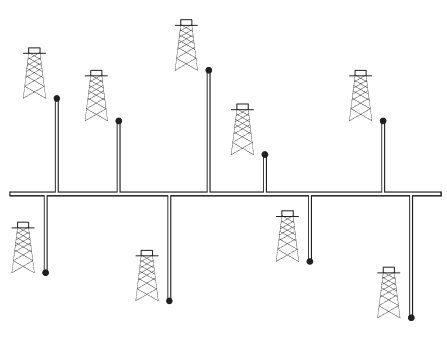
\includegraphics{oilcompany.png}
  \caption{Professor Olay needs to determine the position of the east-west oil pipeline that minimizes the total length of the north-south spurs.}
  \label{fig:oilcompany}
\end{figure}

\section{Professor Olay is consulting for an oil company, which is planning a large pipeline running east to west through an oil field of n wells. The company wants to connect a spur pipeline from each well directly to the main pipeline along a shortest route (either north or south), as shown in Figure \ref{fig:oilcompany}. Given the x-andy-coordinates of the wells, how should the professor pick the optimal location of the main pipeline, which would be the one that minimizes the total length of the spurs? Show how to determine the optimal location in linear time.}

\paragraph{Origin}:
  \subparagraph{Exercise}9.3-9
  \subparagraph{Page}223
\paragraph{Answer}:


\begin{itemize}
  \item If $n$ is odd, we pick the $y$ coordinate of the main pipeline to be equal to the median of all the $y$ coordinates of the wells.
  \item If $n$ is even, we pick the $y$ coordinate of the pipeline to be anything between the $y$ coordinates of the wells with $y$-coordinates which have order statistics $\lfloor (n + 1) / 2 \rfloor$ and the $\lceil (n + 1) / 2 \rceil$. These can all be found in linear time using the algorithm from this section.

\end{itemize}


\section{Bitonic euclidean traveling-salesman problem}

In the \textbf{euclidean traveling-salesman problem},wearegivenasetofn points in the plane, and we wish to find the shortest closed tour that connects all n points. Figure 15.11(a) shows the solution to a 7-point problem. The general problem is NP-hard, and its solution is therefore believed to require more than polynomial time (see Chapter 34).

J. L. Bentley has suggested that we simplify the problem by restricting our attention to \textbf{bitonic tours}, that is, tours that start at the leftmost point, go strictly rightward to the rightmost point, and then go strictly leftward back to the starting point. Figure 15.11(b) shows the shortest bitoni

Describe an $O(n^2)$-time algorithm for determining an optimal bitonic tour. You may assume that no two points have the same x-coordinate and that all operations on real numbers take unit time. (Hint: Scan left to right, maintaining optimal possibilities for the two parts of the tour.)

\paragraph{Origin}:
  \subparagraph{Problems}15-3
  \subparagraph{Page}405
\paragraph{Answer}:



First sort all the points based on their $x$ coordinate. To index our subproblem, we will give the rightmost point for both the path going to the left and the path going to the right. Then, we have that the desired result will be the subproblem indexed by $v$, where $v$ is the rightmost point.

Suppose by symmetry that we are further along on the left-going path, that the leftmost path is going to the $i$th one and the right going path is going until the $j$th one. Then, if we have that $i > j + 1$, then we have that the cost must be the distance from the $i - 1$st point to the ith plus the solution to the subproblem obtained where we replace $i$ with $i - 1$. There can be at most $O(n^2)$ of these subproblem, but solving them only requires considering a constant number of cases. The other possibility for a subproblem is that $j \le i \le j + 1$. In this case, we consider for every $k$ from $1$ to $j$ the subproblem where we replace $i$ with $k$ plus the cost from $k$th point to the $i$th point and take the minimum over all of them. This case requires considering $O(n)$ things, but there are only $O(n)$ such cases. So, the final runtime is $O(n^2)$.


\section{Planning a company party}

Professor Stewart is consulting for the president of a corporation that is planning a company party. The company has a hierarchical structure; that is, the supervisor relation forms a tree rooted at the president. The personnel office has ranked each employee with a conviviality rating, which is a real number. In order to make the party fun for all attendees, the president does not want both an employee and his or her immediate supervisor to attend.

Professor Stewart is given the tree that describes the structure of the corporation, using the left-child, right-sibling representation described in Section 10.4. Each node of the tree holds, in addition to the pointers, the name of an employee and that employee's conviviality ranking. Describe an algorithm to make up a guest list that maximizes the sum of the conviviality ratings of the guests. Analyze the running time of your algorithm.

\paragraph{Origin}:
  \subparagraph{Problems}15-6
  \subparagraph{Page}408
\paragraph{Answer}:

The problem exhibits optimal substructure in the following way: If the root $r$ is included in an optimal solution, then we must solve the optimal subproblems rooted at the grandchildren of $r$. If $r$ is not included, then we must solve the optimal subproblems on trees rooted at the children of $r$. The dynamic programming algorithm to solve this problem works as follows: We make a table $C$ indexed by vertices which tells us the optimal conviviality ranking of a guest list obtained from the subtree with root at that vertex. We also make a table $G$ such that $G[i]$ tells us the guest list we would use when vertex $i$ is at the root. Let $T$ be the tree of guests. To solve the problem, we need to examine the guest list stored at $G[T.root]$. First solve the problem at each leaf $L$. If the conviviality ranking at $L$ is positive, $G[L] = \{L\}$ and $C[L] = L.conviv$. Otherwise $G[L] = \emptyset$ and $C[L] = 0$. Iteratively solve the subproblems located at parents of nodes at which the subproblem has been solved. In general for a node $x$,

$$C[x] = \max(\sum_{y\text{ is a child of } x} C[y], x.conviv + \sum_{y\text{ is a grandchild of } x} C[y]).$$

The runtime is $O(n)$ since each node appears in at most two of the sums (because each node has at most 1 parent and 1 grandparent) and each node is solved once.



\section{Suppose that we have a set of activities to schedule among a large number of lecture halls, where any activity can take place in any lecture hall. We wish to schedule all the activities using as few lecture halls as possible. Give an efficient greedy algorithm to determine which activity should use which lecture hall.}

(This problem is also known as the \textbf{interval-graph coloring problem}. We can create an interval graph whose vertices are the given activities and whose edges connect incompatible activities. The smallest number of colors required to color every vertex so that no two adjacent vertices have the same color corresponds to finding the fewest lecture halls needed to schedule all of the given activities.)

\paragraph{Origin}:
  \subparagraph{Exercise}16.1-4
  \subparagraph{Page}422
\paragraph{Answer}:

Maintain a set of free (but already used) lecture halls $F$ and currently busy lecture halls $B$. Sort the classes by start time. For each new start time which you encounter, remove a lecture hall from $F$, schedule the class in that room, and add the lecture hall to $B$. If $F$ is empty, add a new, unused lecture hall to $F$. When a class finishes, remove its lecture hall from $B$ and add it to $F$. This is optimal for following reason, suppose we have just started using the mth lecture hall for the first time. This only happens when ever classroom ever used before is in $B$. But this means that there are $m$ classes occurring simultaneously, so it is necessary to have $m$ distinct lecture halls in use.

\section{Euler tour}

An \textbf{Euler tour} of a strongly connected, directed graph $G = (V, E)$ is a cycle that traverses each edge of $G$ exactly once, although it may visit a vertex more than once.

\begin{enumerate}
  \item[a] Show that $G$ has an Euler tour if and only if $\text{in-degree}(v) = \text{out-degree}(v)$ for each vertex $v \in V$.
  \item[b] Describe an $O(E)$-time algorithm to find an Euler tour of $G$ if one exists. ($\textit{Hint:}$ Merge edge-disjoint cycles.)
\end{enumerate}

\paragraph{Origin}:
  \subparagraph{Problems}22-3
  \subparagraph{Page}623
\paragraph{Answer}:

\begin{enumerate}
  \item[a] First, we'll show that it is necessary to have in degree equal out degree for each vertex. Suppose that there was some vertex v for which the two were not equal, suppose that $\text{in-degree}(v) - \text{out-degree}(v)$. Note that we may assume that in degree is greater because otherwise we would just look at the transpose graph in which we traverse the cycle backwards. If $v$ is the start of the cycle as it is listed, just shift the starting and ending vertex to any other one on the cycle. Then, in whatever cycle we take going though $v$, we must pass through $v$ some number of times, in particular, after we pass through it a times, the number of unused edges coming out of $v$ is zero, however, there are still unused edges goin in that we need to use. This means that there is no hope of using those while still being a tour, becase we would never be able to escape $v$ and get back to the vertex where the tour started. Now, we show that it is sufficient to have the in degree and out degree equal for every vertex. To do this, we will generalize the problem slightly so that it is more amenable to an inductive approach. That is, we will show that for every graph $G$ that has two vertices $v$ and $u$ so that all the vertices have the same in and out degree except that the indegree is one greater for $u$ and the out degree is one greater for $v$, then there is an Euler path from $v$ to $u$. This clearly lines up with the original statement if we pick $u = v$ to be any vertex in the graph. We now perform induction on the number of edges. If there is only a single edge, then taking just that edge is an Euler tour. Then, suppose that we start at $v$ and take any edge coming out of it. Consider the graph that is obtained from removing that edge, it inductively contains an Euler tour that we can just post-pend to the edge that we took to get out of $v$.
  \item[b] To actually get the Euler circuit, we can just arbitrarily walk any way that we want so long as we don't repeat an edge, we will necessarily end up with a valid Euler tour. This is implemented in the following algorithm, $\text{EULER-TOUR}(G)$ which takes time $O(|E|)$. It has this runtime because the for loop will get run for every edge, and takes a constant amount of time. Also, the process of initializing each edge's color will take time proportional to the number of edges.
\end{enumerate}

\begin{lstlisting}
  EULER-TOUR(G)
  color all edges WHITE
  let (v, u) be any edge
  let L be a list containing v
  while there is some WHITE edge (v, w) coming out of v
      color (v, w) BLACK
      v = w
      append v to L
\end{lstlisting}

\section{Second-best minimum spanning tree}

Let $G = (V, E)$ be an undirected, connected graph whose weight function is $w: E \rightarrow \mathbb{R} $, and suppose that $|E| \ge |V|$ and all edge weights are distinct.

We define a second-best minimum spanning tree as follows. Let $\mathcal T$ be the set of all spanning trees of $G$, and let $T'$ be a minimum spanning tree of $G$. Then a <strong><em>second-best minimum spanning tree</em></strong> is a spanning tree $T$ such that $W(T) = \min_{T'' \in \mathcal T - \{T'\}} \{w(T'')\}$.

\begin{enumerate}
  \item[a] Show that the minimum spanning tree is unique, but that the second-best minimum spanning tree need not be unique.
  \item[b] Let $T$ be the minimum spanning tree of $G$. Prove that $G$ contains edges $(u, v) \in T$ and $(x, y) \notin T$ such that $T - \{(u, v)\} \cup \{(x, y)\}$ is a second-best minimum spanning tree of $G$.
  \item[c] Let $T$ be a spanning tree of $G$ and, for any two vertices $u, v \in V$, let $max[u, v]$ denote an edge of maximum weight on the unique simple path between $u$ and $v$ in $T$. Describe an $O(V^2)$-time algorithm that, given $T$, computes $max[u, v]$ for all $u, v \in V$.
  \item[d] Give an efficient algorithm to compute the second-best minimum spanning tree of $G$.
\end{enumerate}

\paragraph{Origin}:
  \subparagraph{Problems}23-1
  \subparagraph{Page}638
\paragraph{Answer}:

\begin{enumerate}
  \item[a] To see that the second best minimum spanning tree need not be unique, we consider the following example graph on four vertices. Suppose the vertices are $\{a, b, c, d\}$, and the edge weights are as follows:
  
  $$
  \begin{array}{c|c|c|c|c|}
    & a & b & c & d \\
  \hline
  a & - & 1 & 4 & 3 \\
  \hline
  b & 1 & - & 5 & 2 \\
  \hline
  c & 4 & 5 & - & 6 \\
  \hline
  d & 3 & 2 & 6 & - \\
  \hline
  \end{array}
  $$
  
  Then, the minimum spanning tree has weight $7$, but there are two spanning trees of the second best weight, $8$.

  \item[b] We are trying to show that there is a single edge swap that can demote our minimum spanning tree to a second best minimum spanning tree. In obtaining the second best minimum spanning tree, there must be some cut of a single vertex away from the rest for which the edge that is added is not light, otherwise, we would find the minimum spanning tree, not the second best minimum spanning tree. Call the edge that is selected for that cut for the second best minimum spanning tree $(x, y)$. Now, consider the same cut, except look at the edge that was selected when obtaining $T$, call it $(u, v)$. Then, we have that if consider $T - \{(u, v)\} \cup \{(x, y)\}$, it will be a second best minimum spanning tree. This is because if the second best minimum spanning tree also selected a non-light edge for another cut, it would end up more expensive than all the minimum spanning trees. This means that we need for every cut other than the one that the selected edge was light. This means that the choices all align with what the minimum spanning tree was.
  \item[c] We give here a dynamic programming solution. Suppose that we want to find it for $(u, v)$. First, we will identify the vertex $x$ that occurs immediately after $u$ on the simple path from $u$ to $v$. We will then make $\max[u, v]$ equal to the max of $w((u, x))$ and $\max[w, v]$. Lastly, we just consider the case that $u$ and $v$ are adjacent, in which case the maximum weight edge is just the single edge between the two. If we can find $x$ in constant time, then we will have the whole dynamic program running in time $O(V^2)$, since that's the size of the table that's being built up. To find $x$ in constant time, we preprocess the tree. We first pick an arbitrary root. Then, we do the preprocessing for Tarjan's off-line least common ancestors algorithm (See problem 21-3). This takes time just a little more than linear, $O(|V|\alpha(|V|))$. Once we've computed all the least common ancestors, we can just look up that result at some point later in constant time. Then, to find the $w$ that we should pick, we first see if $u = \text{LCA}(u, v)$ if it does not, then we just pick the parent of $u$ in the tree. If it does, then we flip the question on its head and try to compute $\max[v, u]$, we are guaranteed to not have this situation of $v = \text{LCA}(v, u)$ because we know that $u$ is an ancestor of $v$.
  \item[d] We provide here an algorithm that takes time $O(V^2)$ and leave open if there exists a linear time solution, that is a $O(E + V)$ time solution. First, we find a minimum spanning tree in time $O(E + V \lg(V))$, which is in $O(V^2)$. Then, using the algorithm from part c, we find the double array max. Then, we take a running minimum over all pairs of vertices $u$, $v$, of the value of $w(u, v) - \max[u, v]$. If there is no edge between $u$ and $v$, we think of the weight being infinite. Then, for the pair that resulted in the minimum value of this difference, we add in that edge and remove from the minimum spanning tree, an edge that is in the path from $u$ to $v$ that has weight $\max[u, v]$.
\end{enumerate}

\section{Let $G = (V, E)$ be a weighted, directed graph with nonnegative weight function $w: E \rightarrow \{0, 1, \ldots, W\}$ for some nonnegative integer $W$. Modify Dijkstra's algorithm to compute the shortest paths from a given source vertex s in $O(WV + E)$ time.}

\paragraph{Origin}:
  \subparagraph{Exercise}24.3-8
  \subparagraph{Page}664
\paragraph{Answer}:
 
% To modify Dijkstra's algorithm to handle the nonnegative weight function \(w: E \rightarrow \{0, 1, \ldots, W\}\), we can use a bucket-based approach to achieve a time complexity of \(O(WV + E)\). This modification takes advantage of the fact that the weights are integers in a limited range.

% Here are the steps for the modified Dijkstra's algorithm:

\paragraph{Initialize Data Structures}:

\begin{itemize}
  \item Create an array of buckets, where each bucket \(B_i\) is associated with a weight \(i\).
  \item Initialize an array \(dist\) to store the shortest distances from the source vertex to each vertex. Set \(dist[s] = 0\) and \(dist[v] = \infty\) for all other vertices.
  \item Create a priority queue (min-heap) to manage the vertices based on their current distances.
\end{itemize}


\paragraph{Initialization}:
  Insert the source vertex \(s\) into the priority queue with distance \(0\).

\paragraph{Main Loop}:
  Repeat until the priority queue is empty:
  \begin{itemize}
    \item Extract the vertex \(u\) with the minimum distance from the priority queue.
    \item For each outgoing edge \(u \rightarrow v\):
    \begin{itemize}
      \item Calculate the new distance \(alt\) from the source to \(v\) via \(u\): \(alt = dist[u] + w(u \rightarrow v)\).
      \item Update \(dist[v]\) if \(alt < dist[v]\).
      \item If \(dist[v]\) is updated, remove \(v\) from its current bucket and insert it into the bucket corresponding to the new distance \(dist[v]\).
    \end{itemize}
  \end{itemize}

\paragraph{Termination}:
  After the main loop, the array \(dist\) contains the shortest distances from the source vertex to all other vertices.

\paragraph{Time Complexity Analysis}:

\begin{itemize}
  \item Insertion and Deletion in Buckets:
  
  Inserting and deleting vertices from buckets can be done in constant time since the weights are integers in the range \(\{0, 1, \ldots, W\}\).

  \item Priority Queue Operations:
  
  The priority queue operations (insert, extract-min, decrease-key) take \(O(\log V)\) time per operation.

  \item Total Time Complexity:
  
  The main loop runs \(O(V)\) times, and for each iteration, there are \(O(E)\) edge relaxations (constant time per edge relaxation).

  Therefore, the overall time complexity is \(O(WV + E)\).

\end{itemize}

This modification exploits the discrete nature of the weight function, allowing us to organize vertices into buckets based on their distances. The use of buckets helps reduce the time complexity compared to the classic Dijkstra's algorithm when dealing with nonnegative integer weights.

\section{Nesting boxes}

A $d$-dimensional box with dimensions $(x_1, x_2, \ldots, x_d)$ <strong><em>nests</em></strong> within another box with dimensions $(y_1, y_2, \ldots, y_d)$ if there exists a permutation $\pi$ on $\{1, 2, \ldots, d\}$ such that $x_{\pi(1)} < y_1$, $x_{\pi(2)} < y_2$, $\ldots$, $x_{\pi(d)} < y_d$.

\begin{enumerate}
  \item[a] Argue that the nesting relation is transitive.
  \item[b] Describe an efficient method to determine whether or not one $d$-dimensional box nests inside another.
  \item[c] Suppose that you are given a set of $n$ $d$-dimensional boxes $\{B_1, B_2, \ldots, B_n\}$. Give an efficient algorithm to find the longest sequence $\langle B_{i_1}, B_{i_2}, \ldots, B_{i_k} \rangle$ of boxes such that $B_{i_j}$ nests within $B_{i_{j + 1}}$ for $j = 1, 2, \ldots, k - 1$. Express the running time of your algorithm in terms of $n$ and $d$.
\end{enumerate}

\paragraph{Origin}:
  \subparagraph{Problems}24-2
  \subparagraph{Page}678
\paragraph{Answer}:

\begin{enumerate}
  \item[a] Suppose that box $x = (x_1, \dots, x_d)$ nests with box $y = (y_1, \dots, y_d)$ and box $y$ nests with box $z = (z_1, \dots, z_d)$. Then there exist permutations $\pi$ and $\sigma$ such that $x_{\pi(1)} < y_1, \dots, x_{\pi(d)} < y_d$ and $y_{\sigma(1)} < z_1, \dots, y_{\sigma(d)} < z_d$. This implies $x_{\pi(\sigma(1))} < z_1, \dots, x_{\pi(\sigma(d))} < z_d$, so $x$ nests with $z$ and the nesting relation is transitive.
  \item[b] Box $x$ nests inside box $y$ if and only if the increasing sequence of dimensions of $x$ is component-wise strictly less than the increasing sequence of dimensions of $y$. Thus, it will suffice to sort both sequences of dimensions and compare them. Sorting both length $d$ sequences is done in $O(d\lg d)$, and comparing their elements is done in $O(d)$, so the total time is $O(d\lg d)$.
  \item[c] We will create a nesting-graph $G$ with vertices $B_1, \dots, B_n$ as follows. For each pair of boxes $B_i$ , $B_j$, we decide if one nests inside the other. If $B_i$ nests in $B_j$, draw an arrow from $B_i$ to $B_j$. If $B_j$ nests in $B_i$, draw an arrow from $B_j$ to $B_i$. If neither nests, draw no arrow. To determine the arrows efficiently, after sorting each list of dimensions in $O(nd\lg d)$ we compair all pairs of boxes using the algorithm from part (b) in $O(n^2 d)$. By part (a), the resulted graph is acyclic, which allows us to easily find the longest chain in it in $O(n^2)$ in a bottom-up manner. This chain is our answer. Thus, the total time is $O(nd\max(\lg d, n))$.
\end{enumerate}

\section{Show how to express the single-source shortest-paths problem as a product of matrices and a vector. Describe how evaluating this product corresponds to a Bellman-Ford-like algorithm (see Section 24.1).}

\paragraph{Origin}:
  \subparagraph{Exercise}25.1-5
  \subparagraph{Page}692
\paragraph{Answer}:
 
The single-source shortest-paths problem can be expressed as a product of matrices and a vector using the adjacency matrix representation of the graph. Let's consider a directed graph with n vertices and an adjacency matrix \(W\), where \(W[i][j]\) represents the weight of the edge from vertex \(i\) to vertex \(j\). If there is no edge from \(i\) to \(j\), \(W[i][j]\) is set to \(\infty\), and \(W[i][i]\) is set to 0.

The goal is to find the shortest paths from a source vertex \(s\) to all other vertices in the graph.

\paragraph{Matrix Representation}:

Let \(D^{(k)}\) be a matrix representing the shortest path distances after \(k\) iterations, where \(D^{(0)}\) is the initial matrix with only the direct edge weights filled in.

The matrix \(D^{(k)}\) can be computed from \(D^{(k-1)}\) as follows:

\[D^{(k)}[i][j] = \min(D^{(k-1)}[i][j], D^{(k-1)}[i][k] + D^{(k-1)}[k][j])\]

This recurrence relation essentially says that the shortest path from \(i\) to \(j\) either remains the same as in \(D^{(k-1)}\) or becomes shorter by going through vertex \(k\).

\paragraph{Matrix Product and Vector}:

Now, let's define a vector \(d^{(k)}\) representing the shortest path distances after \(k\) iterations. Each element \(d^{(k)}[i]\) represents the shortest distance from the source vertex \(s\) to vertex \(i\) after \(k\) iterations.

The matrix-vector product \(D^{(k)} \times d^{(k)}\) corresponds to updating the shortest path distances after \(k\) iterations.

\[d^{(k)} = D^{(k)} \times d^{(k)}\]

\paragraph{Bellman-Ford-Like Algorithm}:

The product of matrices and vector can be evaluated through a Bellman-Ford-like algorithm. The matrix \(D^{(k)}\) is computed iteratively for \(k = 1\) to \(n-1\), where \(n\) is the number of vertices in the graph.

The algorithm updates the shortest path distances in each iteration, considering the possibility of shorter paths through intermediate vertices. After \(n-1\) iterations, the matrix \(D^{(n-1)}\) represents the shortest path distances.

If there are no negative cycles in the graph, then \(D^{(n-1)}\) contains the correct shortest path distances. If there is a negative cycle, the algorithm can detect it in the \(n\)-th iteration, as any further relaxation in the presence of a negative cycle would lead to shorter and shorter paths indefinitely.

This matrix-vector product approach provides a way to efficiently compute the shortest paths in a graph using matrix operations.

\section{The \textbf{edge connectivity} of an undirected graph is the minimum number $k$ of edges that must be removed to disconnect the graph. For example, the edge connectivity of a tree is $1$, and the edge connectivity of a cyclic chain of vertices is $2$. Show how to determine the edge connectivity of an undirected graph $G = (V, E)$ by running a maximum-flow algorithm on at most $|V|$ flow networks, each having $O(V)$ vertices and $O(E)$ edges.}

\paragraph{Origin}:
  \subparagraph{Exercise}26.2-11
  \subparagraph{Page}731
\paragraph{Answer}:
 
Create an directed version of the graph. Then create a flow network out of it, resolving all antiparallel edges. All edges' capacities are set to $1$. Pick any vertex that wasn't created for antiparallel workaround as the sink and run maximum-flow algorithm with all vertexes that aren't for antipararrel workaround (except the sink) as sources. Find the minimum value out of all $|V| - 1$ maximum flow values.


\section{The \textbf{subgraph-isomorphism problem} takes two undirected graphs $G_1$ and $G_2$, and it asks whether $G_1$ is isomorphic to a subgraph of $G_2$. Show that the subgraphisomorphism problem is $\text{NP-complete}$.}

\paragraph{Origin}:
  \subparagraph{Exercise}34.5-1
  \subparagraph{Page}1100
\paragraph{Answer}:



\paragraph{Subgraph Isomorphism is in NP}:

Given a proposed subgraph of $G_2$ (the subgraph of $G_2$ that we're testing for isomorphism), we can quickly verify in polynomial time whether it is isomorphic to $G_1$. The verification can be done by checking each edge and vertex mapping to ensure that the adjacency relationships are preserved. Therefore, subgraph isomorphism is in NP.

\paragraph{Subgraph Isomorphism is NP-hard}:

To show that the subgraph isomorphism problem is NP-hard, we can reduce the well-known NP-complete problem, the Clique problem, to it. The Clique problem asks whether there exists a clique of size k in a given graph.

The reduction works as follows:

\paragraph{Reduction from Clique to Subgraph Isomorphism}:

Given an instance of the Clique problem with a graph $G$ and an integer $k$, we construct an instance of the subgraph isomorphism problem as follows:

\begin{enumerate}
  \item Let $G_1$ be a complete graph on $k$ vertices (a clique of size $k$).
  \item Let $G_2$ be the input graph $G$.
\end{enumerate}

Now, the question becomes whether there is a subgraph of $G_2$ that is isomorphic to $G_1$ (a clique of size $k$). If we can efficiently solve the subgraph isomorphism problem for this instance, we can solve the Clique problem as well.

\paragraph{Conclusion}:

Since we have shown that subgraph isomorphism is both in NP and NP-hard, it follows that the subgraph isomorphism problem is NP-complete.

\end{document}